\documentclass{supervision}
\usepackage{course}

% Exercises 1-4, 7-9 from Markus's exercise sheet.

\Supervision{1}
\begin{document}

  \emph{Code can be browsed at
  \url{https://github.com/danielchatfield/cst1b-security}}

  \begin{questions}
    \question Decipher the shift cipher text
      \lstinline|LUXDZNUAMNDODJUDTUZDGYQDLUXDGOJDCKDTKKJDOZ|

      \begin{solution}
        \lstinline|FORXTHOUGHXIXDOXNOTXASKXFORXAIDXWEXNEEDXIT|

        \codefile[golang]{code/shift.py}
      \end{solution}

    \question How can you break any transposition cipher with $log_a n$ chosen
      plaintexts, if $a$ is the size of the alphabet and $n$ is the permutation
      block length?

      \begin{solution}
        I'm assuming that the transposition cipher is a block cipher and
        that the chosen plaintext cannot be longer than the permutation block
        length (otherwise it can be trivially cracked with a single plaintext).

        Let $i$ represent the position of a character in the plaintext e.g. if
        a message $M$ is \lstinline|THISISATEST| then $M[i]$ is $H$ if $i=2$.
        And let $j$ represent the position of a character in the ciphertext.

        If we associate a unique ID consisting of characters from the alphabet
        to each position then we can crack the transposition cipher by
        constructing plaintext messages that consist of each character, in
        sequence of the ID. So the first plaintext message would consist of
        the first character of the ID for each position, the second would
        consist of the second etc.

        Since the number of characters required in an alphabet of size $a$ to
        uniquely represent each of $n$ positions is $log_a n$ this is how many
        messages need to be used.

        From the ciphertext you can then work out which position $i$ maps to a
        position $j$ by joining up the characters at that position from each
        ciphertext and looking to see which position had that ID.
      \end{solution}

    \question Show that the shift cipher provides unconditional security if
      $\forall K \in \mathbb{Z}_{26} : \mathbb{P}(K) = 26^{-1}$ for plaintexts
      $M \in \mathbb{Z}_{26}$

      \begin{solution}
        No key is more likely than any other and since the plaintext is a
        single character no statistical analysis on the liklehood of a certain
        plaintext being more likely is possible as each of the 26 different
        plaintexts are equally as nonsensical and thus likely.
      \end{solution}

    \question Show that an encryption scheme (Gen, Enc, Dec) over a message
      space $\mathcal{M}$ is \emph{perfectly secret} if and only if:

      \begin{parts}
        \part for every probability distribution over $\mathcal{M}$, every
          message $M \in \mathcal{M}$, and every ciphertext $C\in
          \mathcal{C}$ with $\mathbb{P}(C) > 0$ we have

          \begin{equation*}
            \mathbb{P}(C|M) = \mathbb{P}(C)
          \end{equation*}

          \begin{solution}
            % TODO
          \end{solution}

        \part for every probability distribution over $\mathcal{M}$, every
          message pair $M_0, M_1 \in \mathcal{M}$, and every ciphertext $C \in
          \mathcal{C}$ with $\mathbb{P}(C) > 0$ we have

          \begin{equation*}
            \mathbb{P}(C|M_0) = \mathbb{P}(C|M_1)
          \end{equation*}

          \begin{solution}
            % TODO
          \end{solution}
      \end{parts}

    \SetQuestionNumber{7}
    \question Using a given pseudo-random function $F : {0,1}^{100} \rightarrow
      {0,1}^{100}$, construct a pseudo-random permutation $P: {0,1}^{300}
      \rightarrow {0,1}^{300}$ by extending the Feistel principle appropriately.

      \begin{solution}
        The Feistel cipher can be extended to accomodate a 3-way split as
        follows:

        Split the plaintext message into 3 equal parts, $L_0$, $C_0$ and $R_0$.

        For each round $i = 0, 1, \ldots , n$, compute

        \begin{align*}
          L_{i+1} &= R_i                     \\
          C_{i+1} &= L_i                     \\
          R_{i+1} &= C_i \oplus F_{k_i}(L_i)
        \end{align*}

        Decryption of a ciphertext is similarly:

        \begin{align*}
          L_{i} &= C_{i+1}                         \\
          C_{i} &= R_{i+1} \oplus F_{k_i}(C_{i+1}) \\
          R_{i} &= L_{i+1}
        \end{align*}

        \begin{center}
          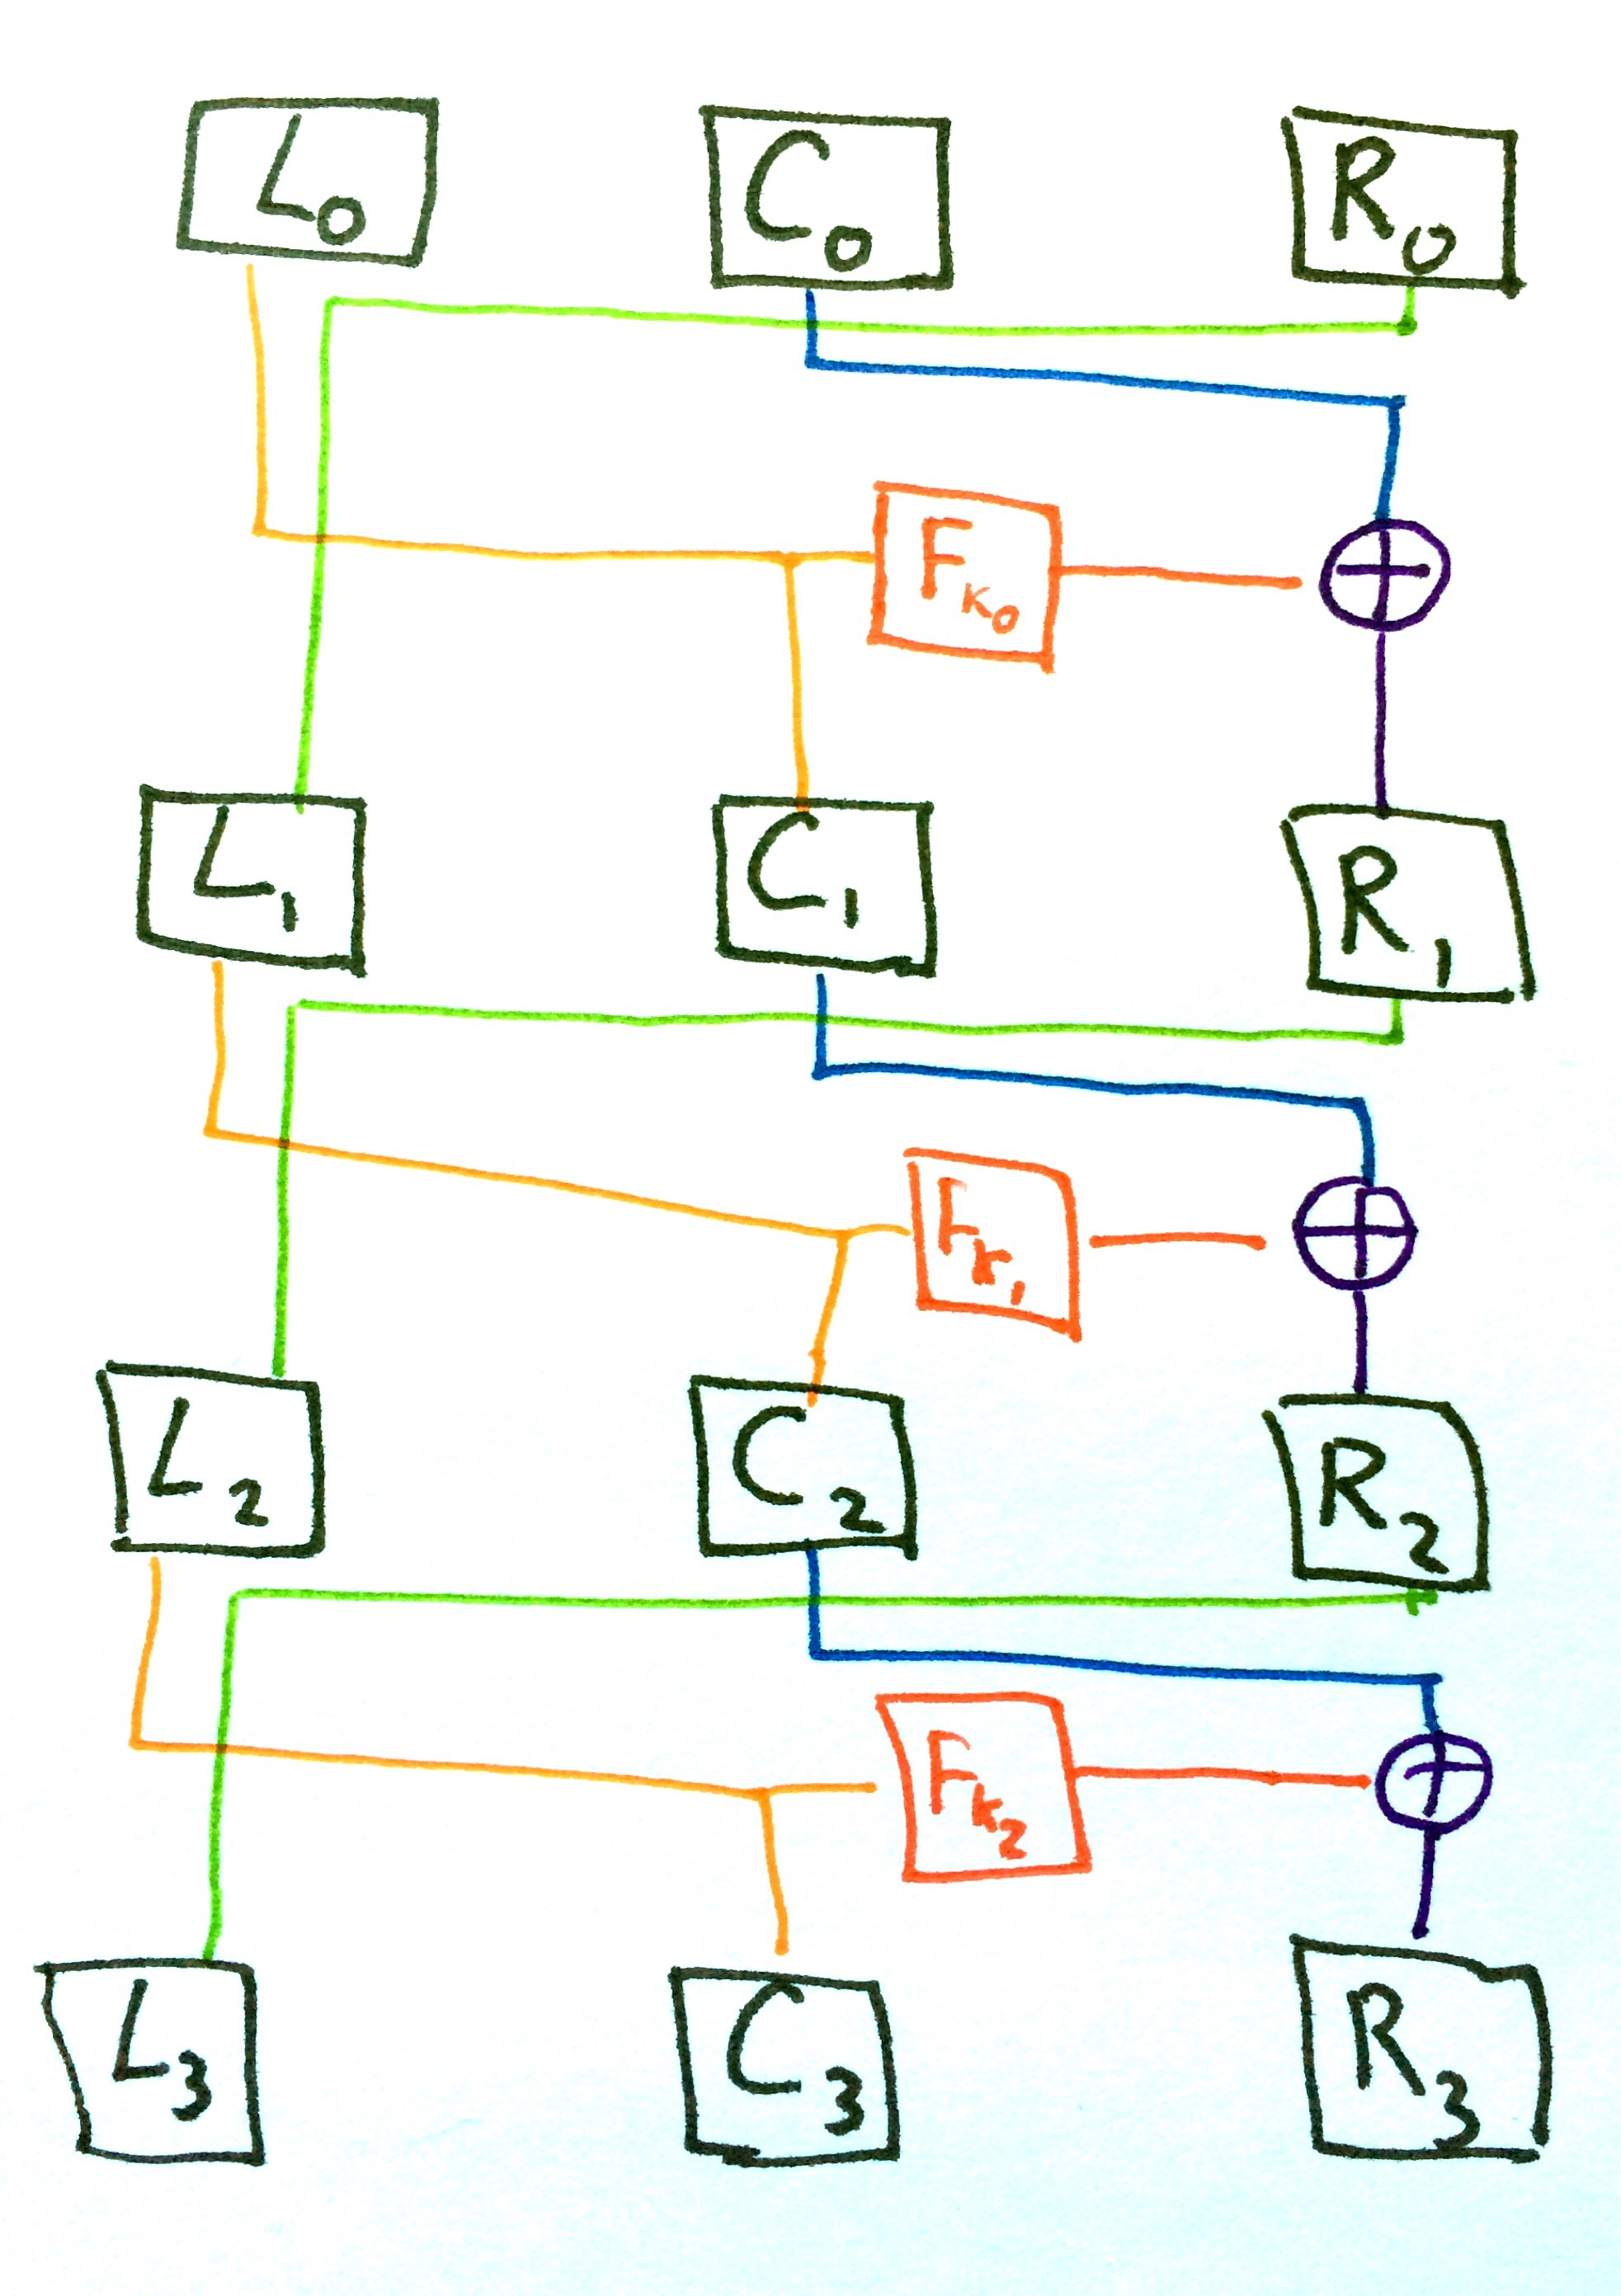
\includegraphics[width=0.5\textwidth]{1-feistel-3}
        \end{center}
      \end{solution}

    \question What happens to the ciphertext block if all bits in both the key
      and plaintext block of DES are inverted.

      \begin{solution}
        The ciphertext block is also inverted.

        Not entirely sure why but kind of makes sense from diagram and
        confirmed programmatically:

        \codefile[golang]{code/inverse-des/cmd.go}
      \end{solution}

    \question Given a hardware implementation of the DES encryption function,
      what has to be modified to make it decrypt.

  \end{questions}
\end{document}
